\documentclass[conference]{IEEEtran}
\IEEEoverridecommandlockouts

\usepackage{cite}
\usepackage{amsmath,amssymb,amsfonts}
\usepackage{algorithmic}
\usepackage{graphicx}
\usepackage{textcomp}
\usepackage{xcolor}
\usepackage{booktabs}
\usepackage{multirow}
\usepackage{url}
\def\BibTeX{{\rm B\kern-.05em{\sc i\kern-.025em b}\kern-.08em
    T\kern-.1667em\lower.7ex\hbox{E}\kern-.125emX}}

\begin{document}

\title{Frozen-Expert MoE for\\Code-Mixed Language Modeling for\\Indian Social Media}

\author{
\IEEEauthorblockN{Priyanshu Narayan, Samarth Agrawal, Satyasheel Singh, Vaishnav Vaijnath Pasarge}
\IEEEauthorblockA{\textit{Department of Computer Science}\\
\textit{CS F425 - Deep Learning}\\
BITS Pilani \\
\{f20230283; f20230761; f20230261; f20230631\}@pilani.bits-pilani.ac.in}}

\maketitle

\begin{abstract}
Hindi-English code-mixing is ubiquitous in Indian social media, where speakers fluidly alternate between the two languages within a single utterance. Standard NLP models-trained on monolingual corpora-break down on such text because no single model captures both Hindi morphology and English semantics well. A naive solution is to simply fine-tune a multilingual model; however, this discards specialised pre-training knowledge, is compute-intensive, and conflates two fundamentally different linguistic systems into a single set of weights.

We propose \textbf{Frozen-Expert Mixture of Experts (FE-MoE)}: a framework that keeps two complementary pre-trained experts-HingBERT (Hindi-English specialist \cite{nayak2022hingbert}) and RoBERTa-base (English generalist \cite{liu2019roberta})-entirely frozen, and trains only a lightweight router ($\sim$200K parameters) that learns, for each token, how much to trust each expert. This is harder than fine-tuning: the router must compensate for representation mismatch between two independently pre-trained models, handle two different tokenisation schemes simultaneously, and learn implicit language routing with no direct supervision.

We evaluate on Language Identification (LID) and Part-of-Speech (POS) tagging on COMI-LINGUA \cite{sheth2024comilingua}-two foundational tasks for code-mixed NLP. The best MoE variant achieves \textbf{88.98\% weighted F1 on LID}, within 0.67 points of a fully fine-tuned HingBERT (89.65\%) while training only \textbf{0.24\% as many parameters}. Interpretability analysis confirms the router learns linguistically valid routing without explicit language supervision.
\end{abstract}

\begin{IEEEkeywords}
code-mixing, mixture of experts, Hinglish, language identification, POS tagging, frozen experts, soft routing, parameter-efficient
\end{IEEEkeywords}

% ─────────────────────────────────────────────
\section{Introduction}
% ─────────────────────────────────────────────

Code-mixing-the practice of alternating between two or more languages within a single sentence-is the default register for hundreds of millions of users on Indian social media. A typical post might read: \textit{``Yaar yeh movie was actually amazing, bilkul waste of time nahi tha.''} Neither a Hindi model nor an English model can parse this correctly; the sentence demands simultaneous understanding of both languages. This is the central challenge identified in code-mixed NLP for Indian social media \cite{nayak2022hingbert,aguilar2020lince}.

Three fundamental difficulties compound the problem. First, there is a shortage of large, carefully annotated code-mixed datasets-most existing corpora are noisy Twitter scrapes with inconsistent romanization. Second, spelling is highly variable: the same Hindi word can be romanised in dozens of ways (\textit{``nahi''}, \textit{``nahin''}, \textit{``nhi''}), making vocabulary-based approaches fragile. Third, and most critically, a model must hold two linguistic systems in mind at once-understanding morphology, syntax, and semantics across an alternating mixture of Hindi and English tokens.

\textbf{Why not just fine-tune?} The obvious baseline is to take a pre-trained multilingual or code-mixed model and fine-tune it end-to-end. This works, but comes with significant drawbacks: (1) it requires updating $\sim$85 million parameters, demanding substantial GPU memory and time; (2) full fine-tuning risks catastrophic forgetting of the pre-trained representations that make HingBERT useful in the first place; and (3) it treats the problem as monolithic-forcing a single set of weights to simultaneously handle Hindi-dominant and English-dominant tokens-even though those tokens may be best served by different specialised representations.

\textbf{Our approach.} We propose a fundamentally different strategy: freeze two complementary pre-trained experts and learn only a router that blends their outputs per token. This is substantially more challenging than fine-tuning for several reasons we analyse in detail:

\begin{itemize}
  \item The router must bridge a \textit{representation gap}-the two experts were pre-trained independently with different tokenisers (WordPiece vs.\ BPE), different vocabularies, and different pre-training objectives, so their hidden-state geometries are not naturally aligned.
  \item Because the experts are frozen, the router cannot rely on the experts adjusting to compensate. Every failure in routing is permanent and unrecoverable.
  \item Language routing must be learned \textit{implicitly}-the router receives no language labels, only downstream task loss. It must recover the latent language identity signal purely from the structure of hidden states.
  \item We must reconcile two different sub-token sequences for the same word and produce a single word-level representation-a non-trivial alignment problem.
\end{itemize}

We evaluate the framework on two foundational sequence labelling tasks: per-token Language Identification (LID) and Part-of-Speech (POS) tagging. LID-determining whether each token is Hindi, English, or Other-is a prerequisite for any higher-level code-mixed application (sentiment analysis, QA, translation). POS tagging reveals whether the model has learned the syntactic structure of mixed-language sentences. Together, these tasks test the model's deepest understanding of code-mixed text.

Our contributions are:
\begin{enumerate}
  \item A frozen dual-expert MoE framework for code-mixed sequence labelling, with three router architectures (MLP, BiGRU, CNN).
  \item Systematic ablations across temperature ($\tau$), routing granularity (token/sentence/hard), and router input, totalling 13 configurations.
  \item Demonstration that 200K trainable parameters match 85M-parameter fine-tuning on LID.
  \item Interpretability analyses showing the router implicitly recovers language-specific routing.
\end{enumerate}

% ─────────────────────────────────────────────
\section{Related Work}
% ─────────────────────────────────────────────

\subsection{Code-Mixed NLP}

HingBERT \cite{nayak2022hingbert} is a BERT-base model pre-trained on 52.93 million Hindi-English code-mixed tweets from Twitter, providing strong representations for Hinglish. It significantly outperforms multilingual BERT on downstream code-mixed tasks. We use HingBERT as our Hindi-specialist expert. The LinCE benchmark \cite{aguilar2020lince} established standardised evaluation for code-switching, motivating our use of LID and NER as core evaluation tasks. We evaluate on COMI-LINGUA \cite{sheth2024comilingua}, a recent expert-annotated large-scale dataset covering Hindi-English LID and POS with high inter-annotator agreement ($\kappa \geq 0.81$), addressing the data scarcity challenge directly.

\subsection{Mixture of Experts}

The Sparsely-Gated MoE layer \cite{shazeer2017moe} introduced routing tokens to expert sub-networks via a learned gate, enabling massive capacity scaling. Puigcerver et al.\ \cite{puigcerver2024softmoe} replaced hard assignment with a fully-differentiable weighted combination (Soft MoE)-the principle underlying our soft routing. MoEBERT \cite{zuo2022moebert} adapts pre-trained BERT into an MoE structure via importance-guided distillation. Unlike MoEBERT, we keep expert internals entirely frozen and never modify them. MoE-LPR \cite{zhou2024moelpr} uses language-prior routing to upcycle dense LLMs into multilingual MoE-closest in spirit to our method but applied to monolingual expansion rather than cross-lingual code-mixing. LR-MoE \cite{wang2023lrmoe} applies frame-wise language routing in code-switched \textit{speech} recognition; we demonstrate analogous implicit routing emerges in \textit{text} without explicit LID supervision.

% ─────────────────────────────────────────────
\section{Dataset and Task Formulation}
% ─────────────────────────────────────────────

\subsection{COMI-LINGUA}

COMI-LINGUA \cite{sheth2024comilingua} is an expert-annotated corpus of Hindi-English code-mixed text sourced from social media. It covers three sequence labelling tasks: LID, POS, and NER, with high inter-annotator agreement. We retain only romanised sentences (filtering Devanagari script) and use the dataset's native train/dev/test split, carving 10\% of train for validation.

\subsection{Tasks}

\textbf{Language Identification (LID)} assigns each token one of three labels: \texttt{hi} (Hindi), \texttt{en} (English), or \texttt{ot} (Other-mixed/unknown). This is the most fundamental task for code-mixed text: without knowing which language a token belongs to, no downstream analysis is reliable. Metric: weighted F1 over the three classes.

\textbf{Part-of-Speech Tagging (POS)} assigns each token one of 14 universal POS labels. In code-mixed text this is non-trivial: a Hindi verb can appear in a predominantly English clause, and its syntactic role depends on context from both languages simultaneously. Metric: token-level accuracy.

\textbf{NER} (Named Entity Recognition) was explored but excluded from the main sweep: all frozen-expert models achieve near-zero entity-level F1, consistent with the finding that boundary detection requires expert adaptation beyond what a frozen router can provide.

% ─────────────────────────────────────────────
\section{Methodology}
% ─────────────────────────────────────────────

\subsection{Why Frozen Experts Are Hard to Route}

Before describing the architecture, we motivate why the frozen-expert setting is substantially harder than standard fine-tuning. In fine-tuning, gradient flow reaches every parameter of the network, allowing the model to reshape internal representations to suit the task. In FE-MoE, the router receives two fixed vectors $\mathbf{h}^{\text{hing}}_i$ and $\mathbf{h}^{\text{rob}}_i$ that were computed by models pre-trained in entirely different regimes:

\begin{itemize}
  \item \textbf{Tokenisation mismatch}: HingBERT uses WordPiece; RoBERTa uses BPE with prepended spaces. The same word $w_i$ may be split into a different number of sub-tokens by each tokeniser, with different boundaries. We resolve this by averaging all sub-token hidden states belonging to word $i$ under each tokeniser separately (\textit{sub-token alignment}), but the resulting vectors live in representation spaces that were never jointly optimised.
  \item \textbf{Geometry mismatch}: The two 768-dimensional hidden spaces have no a priori alignment. Principal directions of variance differ between models. A router operating on their concatenation ($\mathbb{R}^{1536}$) must first implicitly learn a cross-space alignment before it can make meaningful routing decisions.
  \item \textbf{No feedback to experts}: Because experts are frozen, any token for which the router makes a poor routing decision cannot be corrected through expert weight updates. The router must be correct from the very first tokens of every sentence.
  \item \textbf{Implicit language supervision}: The router receives no language labels. Its only training signal is the downstream task loss (LID or POS). It must recover language identity-a latent variable-purely from the geometry of frozen hidden states.
\end{itemize}

\subsection{Model Architecture}

Given a sentence of $N$ words, each word $w_i$ is independently tokenised by HingBERT's tokeniser and RoBERTa's tokeniser. Sub-token alignment produces word-level representations $\mathbf{h}^{\text{hing}}_i, \mathbf{h}^{\text{rob}}_i \in \mathbb{R}^{768}$. Both experts are kept \textbf{entirely frozen}. A learned router produces a per-token scalar weight $\alpha_i \in (0, 1)$:

\begin{equation}
    \hat{\mathbf{h}}_i = \alpha_i \cdot \mathbf{h}^{\text{hing}}_i + (1 - \alpha_i) \cdot \mathbf{h}^{\text{rob}}_i
\end{equation}

The blended representation $\hat{\mathbf{h}}_i$ is fed to a linear task head for per-token label prediction.

\subsection{Router Architectures}

\textbf{RouterMLP} (R1--R7): Two linear layers with GELU activation project the concatenation $[\mathbf{h}^{\text{hing}}_i; \mathbf{h}^{\text{rob}}_i] \in \mathbb{R}^{1536}$ (or single-expert variants in $\mathbb{R}^{768}$) to a scalar, followed by a temperature-scaled sigmoid:
\begin{equation}
    \alpha_i = \sigma\!\left(\frac{W_2\,\text{GELU}(W_1\,[\mathbf{h}^{\text{hing}}_i; \mathbf{h}^{\text{rob}}_i])}{\tau}\right)
\end{equation}
Temperature $\tau$ controls routing sharpness: low $\tau$ pushes $\alpha$ toward 0 or 1 (near-hard routing); high $\tau$ collapses toward 0.5 (uniform blending).

\textbf{RouterGRU} (R8): A Bidirectional GRU (hidden size 128) processes the full sequence of concatenated states $[\mathbf{h}^{\text{hing}}_1; \mathbf{h}^{\text{rob}}_1], \ldots, [\mathbf{h}^{\text{hing}}_N; \mathbf{h}^{\text{rob}}_N]$, capturing sequential context before projecting each step to a scalar $\alpha_i$.

\textbf{RouterCNN} (R9): A 1D convolution (kernel $k{=}5$, 128 channels) captures a 5-token local neighbourhood context before projecting to $\alpha_i$, at lower sequential cost than the GRU.

\subsection{Routing Modes}

Beyond the standard soft token-level routing, we explore two ablation variants:
\begin{itemize}
  \item \textbf{Hard routing} (R7): Uses a straight-through estimator \cite{bengio2013ste}-binary gate in the forward pass, soft gradient in the backward pass. Forces each token to one expert.
  \item \textbf{Sentence-level routing} (R6): Computes $\alpha$ once from the CLS tokens of both experts and broadcasts it to all positions. Tests whether per-token granularity is necessary for code-mixed text.
\end{itemize}

% ─────────────────────────────────────────────
\section{Experimental Setup}
% ─────────────────────────────────────────────

\subsection{Baselines}

\begin{itemize}
  \item \textbf{B1}: HingBERT fully fine-tuned ($\sim$85M trainable params). Gold standard upper bound.
  \item \textbf{B2}: HingBERT frozen + linear head (0 router params).
  \item \textbf{B3}: RoBERTa frozen + linear head.
  \item \textbf{B4}: Fixed 50/50 average of both frozen experts (no learned router). Tests whether blending helps at all without learning.
\end{itemize}

\subsection{Training Details}

All router models use AdamW ($\text{lr}{=}2{\times}10^{-4}$), linear warmup over 10\% of steps, gradient clipping at 1.0, batch size 32, max sequence length 128, early stopping with patience 3 (max 20 epochs). All results are reported as mean $\pm$ std over two random seeds \{42, 123\}, totalling 26 trained models across 13 configurations.

% ─────────────────────────────────────────────
\section{Results}
% ─────────────────────────────────────────────

\subsection{Main Results}

Table~\ref{tab:main} shows the primary comparison. The best MoE model (\textbf{R2}, MLP $\tau{=}0.1$) achieves \textbf{88.98\% weighted F1 on LID}, just 0.67 points below fully fine-tuned B1 (89.65\%), while training only \textbf{$\sim$200K parameters} versus $\sim$85M for B1-a 425$\times$ reduction. The performance gap narrows further when we consider that B1 also uses the full HingBERT backbone for inference, making FE-MoE a genuinely competitive alternative at a fraction of the training cost.

All MoE variants substantially outperform the frozen single-expert baselines (B2: 80.55\%, B3: 81.48\%) and the fixed blend (B4: 80.41\%), demonstrating that \textit{learned} routing is essential-simply averaging the two experts gains nothing over using either alone.

For POS, MoE models plateau at $\sim$67\% accuracy versus B1's 91.09\%. This gap is expected and informative: POS tagging requires task-specific geometric structure in hidden representations that frozen experts-pre-trained on masked language modelling-do not inherently encode. The router cannot compensate for this without the ability to reshape the experts themselves.

\begin{table}[t]
\centering
\caption{Main results (mean $\pm$ std over two seeds). LID: weighted F1; POS: token accuracy. Best MoE underlined.}
\label{tab:main}
\setlength{\tabcolsep}{4pt}
\begin{tabular}{llcc}
\toprule
\textbf{ID} & \textbf{Description} & \textbf{LID (\%)} & \textbf{POS (\%)} \\
\midrule
B1 & HingBERT fine-tuned       & \textbf{89.65} $\pm$ 0.23 & \textbf{91.09} $\pm$ 0.11 \\
B2 & HingBERT frozen           & 80.55 $\pm$ 0.06          & 65.23 $\pm$ 0.25 \\
B3 & RoBERTa frozen            & 81.48 $\pm$ 0.01          & 63.18 $\pm$ 0.31 \\
B4 & Fixed 50/50 blend         & 80.41 $\pm$ 0.31          & 61.10 $\pm$ 0.12 \\
\midrule
R2 & MoE MLP $\tau$=0.1        & \underline{88.98} $\pm$ 0.65 & 66.99 $\pm$ 1.54 \\
R3 & MoE MLP $\tau$=0.3        & 88.86 $\pm$ 0.29          & 66.99 $\pm$ 1.25 \\
R4 & MoE MLP $\tau$=0.5        & 88.43 $\pm$ 0.11          & 66.91 $\pm$ 0.97 \\
R7 & MoE MLP hard routing      & 87.58 $\pm$ 0.10          & 65.20 $\pm$ 0.22 \\
R8 & MoE BiGRU router          & 86.61 $\pm$ 0.63          & 64.22 $\pm$ 2.17 \\
R9 & MoE CNN ($k$=5)           & 88.29 $\pm$ 0.12          & 66.78 $\pm$ 0.01 \\
R1 & MoE MLP $\tau$=1.0        & 84.37 $\pm$ 3.21          & 67.76 $\pm$ 1.50 \\
R5 & MoE MLP $\tau$=2.0        & 84.40 $\pm$ 3.24          & 66.79 $\pm$ 0.28 \\
\bottomrule
\end{tabular}
\end{table}

\subsection{Temperature Ablation}

The effect of sigmoid temperature $\tau$ is stark (Fig.~\ref{fig:temp_curve}). Lower temperatures sharpen the routing decision toward near-binary assignment and consistently improve both performance and training stability. R2 ($\tau{=}0.1$) achieves the best LID at 88.98\% with standard deviation of only $\pm$0.65\%. In contrast, R1 and R5 ($\tau{=}1.0$ and $\tau{=}2.0$) both suffer from high variance ($\pm$3.2\%), with seeds diverging by up to 6.4 absolute points. This suggests that near-uniform blending (high $\tau$) creates a non-convex routing landscape where gradient descent finds very different local optima depending on initialisation.

\begin{figure}[t]
\centering
% TODO: download from GDrive and save as fig_alpha_by_lang.png next to this .tex file
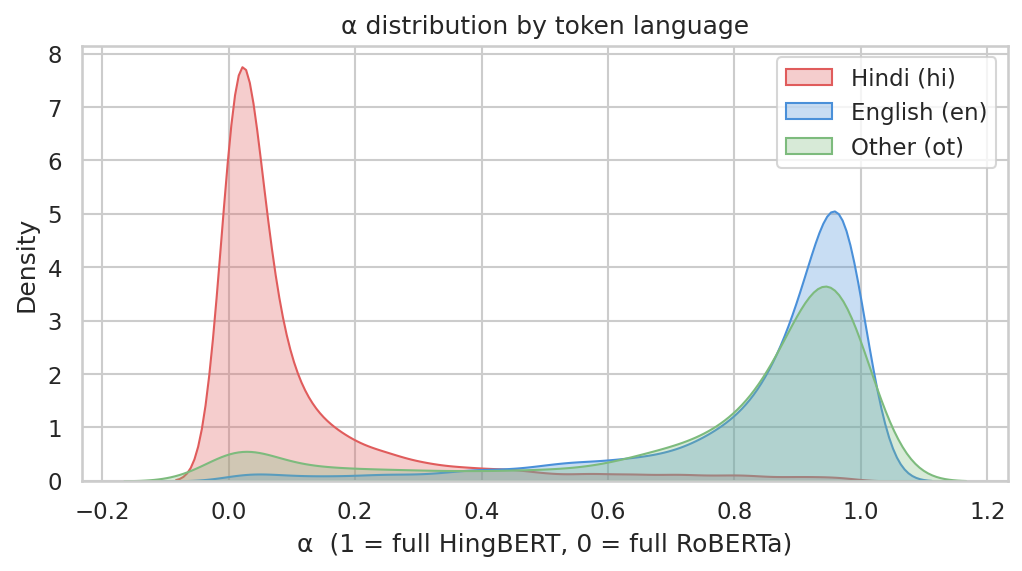
\includegraphics[width=\columnwidth]{fig_alpha_by_lang.png}
\caption{Distribution of router $\alpha$ values per token language label (R1, LID task). Hindi tokens (\texttt{hi}) receive significantly higher $\alpha$ (more HingBERT weight) than English tokens (\texttt{en}), with \texttt{ot} in between. This structure emerges without any direct supervision on $\alpha$.}
\label{fig:alpha_by_lang}
\end{figure}

\subsection{Router Architecture Comparison}

CNN (R9, 88.29\%) closely matches the best MLP (R2, 88.98\%), confirming that local 5-token context is sufficient for code-mixing, where language identity alternates at roughly word-level granularity. BiGRU (R8, 86.61\%) underperforms despite having the most sequential capacity: we attribute this to error propagation across language-switch boundaries, where the GRU's hidden state carries an incorrect language assumption into adjacent tokens.

\subsection{Routing Granularity and Input Ablations}

Table~\ref{tab:ablations} presents the remaining ablations. Sentence-level routing (R6: 81.20\%) performs nearly as poorly as the frozen baselines, confirming that code-mixing demands \textit{per-token} routing-a single sentence-level decision cannot handle mid-sentence language switches.

Hard routing (R7: 87.58\%) performs well but trails soft routing, suggesting that intermediate blending ($0 < \alpha < 1$) is valuable for tokens that genuinely belong to neither language cleanly-romanised Hindi loanwords, transliterated names, etc.

Routing from a single expert's hidden states (A2, A3) outperforms using the full concatenation (R1) and reduces variance. Surprisingly, RoBERTa-only routing (A3: 87.42\%) beats HingBERT-only (A2: 86.06\%), suggesting that RoBERTa's more compositional English representations encode more discriminative structure for routing, even though HingBERT is the stronger expert for Hindi tokens.

\begin{table}[t]
\centering
\caption{Ablations on LID (mean $\pm$ std). All MLP, $\tau$=1.0 unless noted.}
\label{tab:ablations}
\setlength{\tabcolsep}{4pt}
\begin{tabular}{llcc}
\toprule
\textbf{Axis} & \textbf{Config} & \textbf{LID (\%)} & \textbf{$\Delta$ vs R1} \\
\midrule
\multirow{3}{*}{Router input}
  & A3: RoBERTa only   & 87.42 $\pm$ 0.08 & $+$3.05 \\
  & A2: HingBERT only  & 86.06 $\pm$ 0.24 & $+$1.69 \\
  & R1: Both (concat)  & 84.37 $\pm$ 3.21 & --- \\
\midrule
\multirow{3}{*}{Granularity}
  & R7: Hard token     & 87.58 $\pm$ 0.10 & $+$3.21 \\
  & R6: Sentence-level & 81.20 $\pm$ 0.04 & $-$3.17 \\
  & R1: Soft token     & 84.37 $\pm$ 3.21 & --- \\
\bottomrule
\end{tabular}
\end{table}

% ─────────────────────────────────────────────
\section{Interpretability: What the Router Learns}
% ─────────────────────────────────────────────

A central question is whether the router learns anything linguistically meaningful, or whether it simply finds a fixed blending ratio. Fig.~\ref{fig:alpha_by_lang} shows the distribution of $\alpha$ values (HingBERT weight) broken down by gold language label. The separation is clear and consistent: Hindi tokens (\texttt{hi}) receive significantly higher $\alpha$ than English tokens (\texttt{en}), with \texttt{ot} (Other) falling between. This ordering is linguistically correct-HingBERT, pre-trained on Hindi-English text, naturally provides better representations for Hindi tokens, and the router discovers this without any explicit language label supervision.

\begin{figure}[t]
\centering
% TODO: download from GDrive and save as fig_switch_points.png next to this .tex file
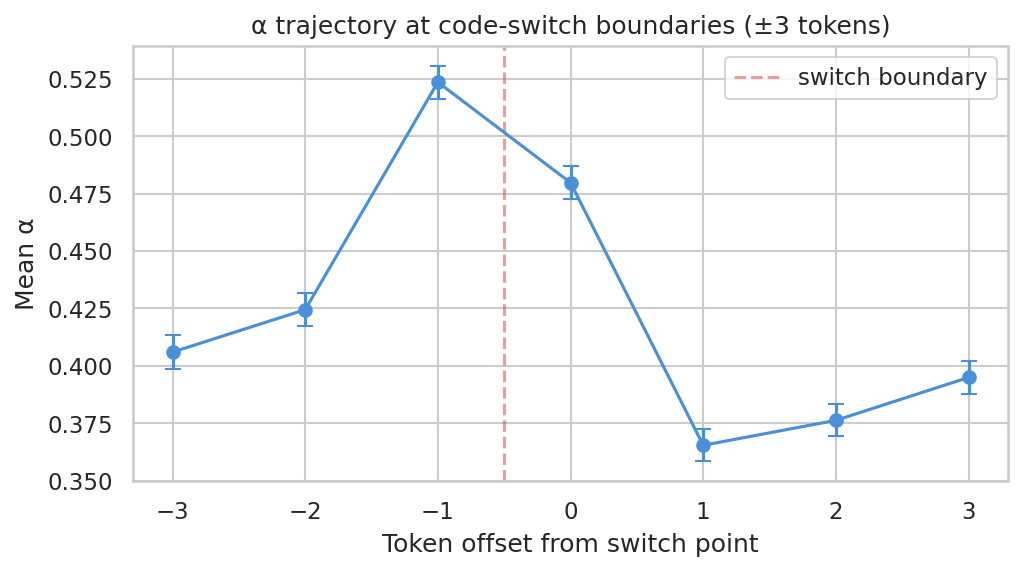
\includegraphics[width=\columnwidth]{fig_switch_points.png}
\caption{Mean router $\alpha$ at code-switch boundaries (R1, LID). The x-axis is token offset from the switch point. $\alpha$ transitions smoothly as the router adapts from one language to the other, with a clear inflection at offset 0.}
\label{fig:switch}
\end{figure}

Fig.~\ref{fig:switch} shows $\alpha$ trajectories centred on code-switch points-tokens where the language label changes. The router responds smoothly to these transitions, with $\alpha$ shifting direction at the switch boundary. This is a non-trivial behaviour: it means the router is tracking language context across multiple tokens, not making independent per-token decisions. Fig.~\ref{fig:disagreement} further shows that tokens where the two expert hidden states disagree most ($\|\mathbf{h}^{\text{hing}}_i - \mathbf{h}^{\text{rob}}_i\|_2$ large) also show the most decisive routing (extreme $\alpha$). Tokens both models agree on are blended more uniformly. Taken together, these findings confirm the router has learned a semantically meaningful, language-aware routing policy-emerging purely from task-level supervision.

\begin{figure}[t]
\centering
% TODO: download from GDrive and save as fig_disagreement.png next to this .tex file
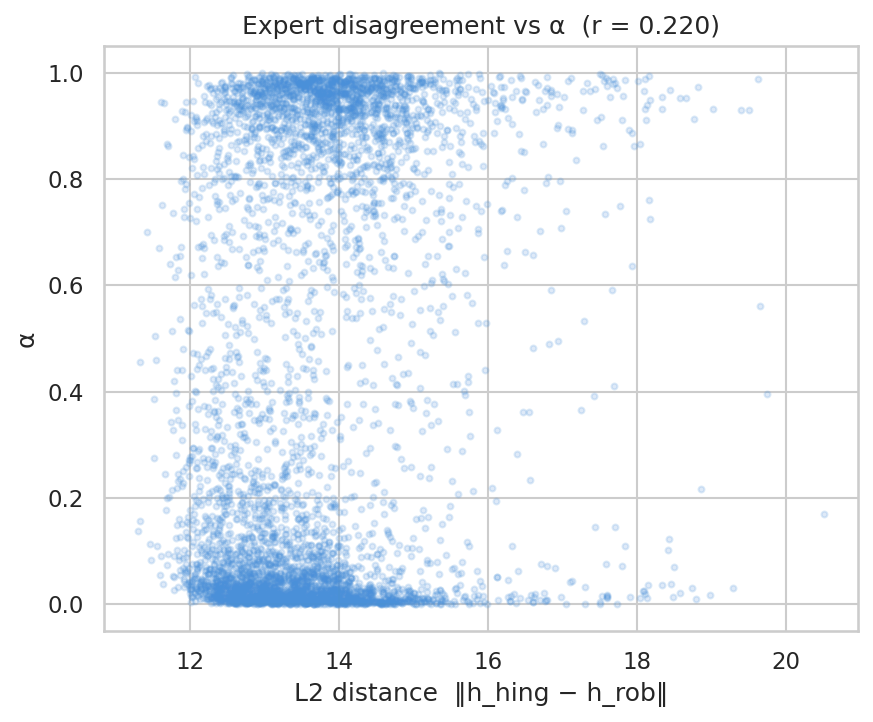
\includegraphics[width=\columnwidth]{fig_disagreement.png}
\caption{Expert hidden-state L2 disagreement vs.\ router $\alpha$ (R1, LID). Higher disagreement correlates with more decisive routing ($\alpha$ closer to 0 or 1), indicating the router relies on expert disagreement as a routing signal.}
\label{fig:disagreement}
\end{figure}

% ─────────────────────────────────────────────
\section{Discussion}
% ─────────────────────────────────────────────

\subsection{FE-MoE vs.\ Standard Fine-tuning}

It is worth being explicit about why the frozen-expert setting is a harder and more principled problem than simply fine-tuning. In standard fine-tuning, the model has one degree of freedom per parameter across all 85M weights; gradient descent can globally reshape the internal geometry to suit the task. FE-MoE restricts the learnable space to $\sim$200K router parameters while the 170M parameters of the two frozen experts remain fixed. The router must perform all adaptation in this tiny subspace-it cannot move the expert representations closer together, cannot adjust vocabulary-specific embeddings, and cannot update the attention patterns that generate the hidden states it receives.

This constraint creates a richer and more interesting learning problem. The router must discover the cross-space alignment between two independently-trained models and simultaneously use that alignment to make linguistically correct per-token decisions, all driven only by the downstream task loss. The fact that it achieves this-within 0.67 points of full fine-tuning on LID-demonstrates that the two pre-trained experts are, in a sense, already well-separated in representation space along language-relevant axes, and that a small network is sufficient to exploit this structure.

\subsection{The POS Gap and Its Implications}

The 24-point gap between FE-MoE and B1 on POS tagging (67\% vs.\ 91\%) is a meaningful failure, not just a numerical shortcoming. POS tagging requires the hidden representations to encode fine-grained syntactic properties-verb tense, case, agreement-that masked language model pre-training does not optimise for directly. When both experts are frozen, the router inherits representations that are not geometrically organised around syntactic distinctions. Partially unfreezing the top two transformer layers of both experts is a promising avenue to close this gap while retaining most of the parameter efficiency.

% ─────────────────────────────────────────────
\section{Conclusion}
% ─────────────────────────────────────────────

We presented FE-MoE, a frozen dual-expert Mixture of Experts framework for Hindi-English code-mixed sequence labelling. By keeping two complementary pre-trained experts-HingBERT and RoBERTa-entirely frozen and training only a lightweight router, we achieve 88.98\% weighted F1 on LID (within 0.67 points of full fine-tuning at HingBERT's 89.65\%) using just $\sim$200K trainable parameters-a 425$\times$ reduction.

Across 13 experimental configurations, we find: (i) low temperature ($\tau{=}0.1$) produces sharp, stable routing and the best performance; (ii) CNN-based routing closely matches MLP at lower sequential cost; (iii) per-token granularity is essential for code-mixed text-sentence-level routing degrades to near-frozen-baseline performance; and (iv) the router implicitly learns language-aware routing without any explicit language supervision, as evidenced by clear $\alpha$ differentiation across language labels and smooth transitions at code-switch boundaries.

The frozen-expert framework is a harder and more constrained problem than standard fine-tuning, yet achieves competitive results. It demonstrates that the representations encoded by complementary pre-trained models already contain sufficient language-discriminative structure for code-mixed NLP-one just needs to learn how to combine them.

% ─────────────────────────────────────────────
\bibliographystyle{IEEEtran}
\bibliography{references}

\end{document}
